\section{Konkrete Architektur}
\textcolor{blue}{\textit{In diesem Abschnitt werden die zuvor identifizierten Schnittstellen der Komponenten genauer beschrieben. Im Komponentendiagramm werden daher Abhängigkeiten und Implementierungsbeziehungen beschrieben bzw. ergänzt.
}}

\begin{figure}[H]
\centering
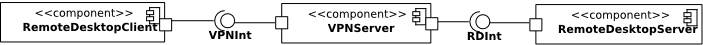
\includegraphics[width=1\textwidth]{img/KomponentendiagrammKonkret.png}
\caption{\textcolor{blue}{Durch eigenes Komponentendiagramm ersetzen}}
\label{KomponentendiagrammKonkret}
\end{figure}
